\chapter{Umsetzung einer Pseudo-Navigation}
\label{chap:5}

\begin{wrapfigure}{R}{0.6\textwidth}
	\vspace{-\baselineskip}
	\centering
	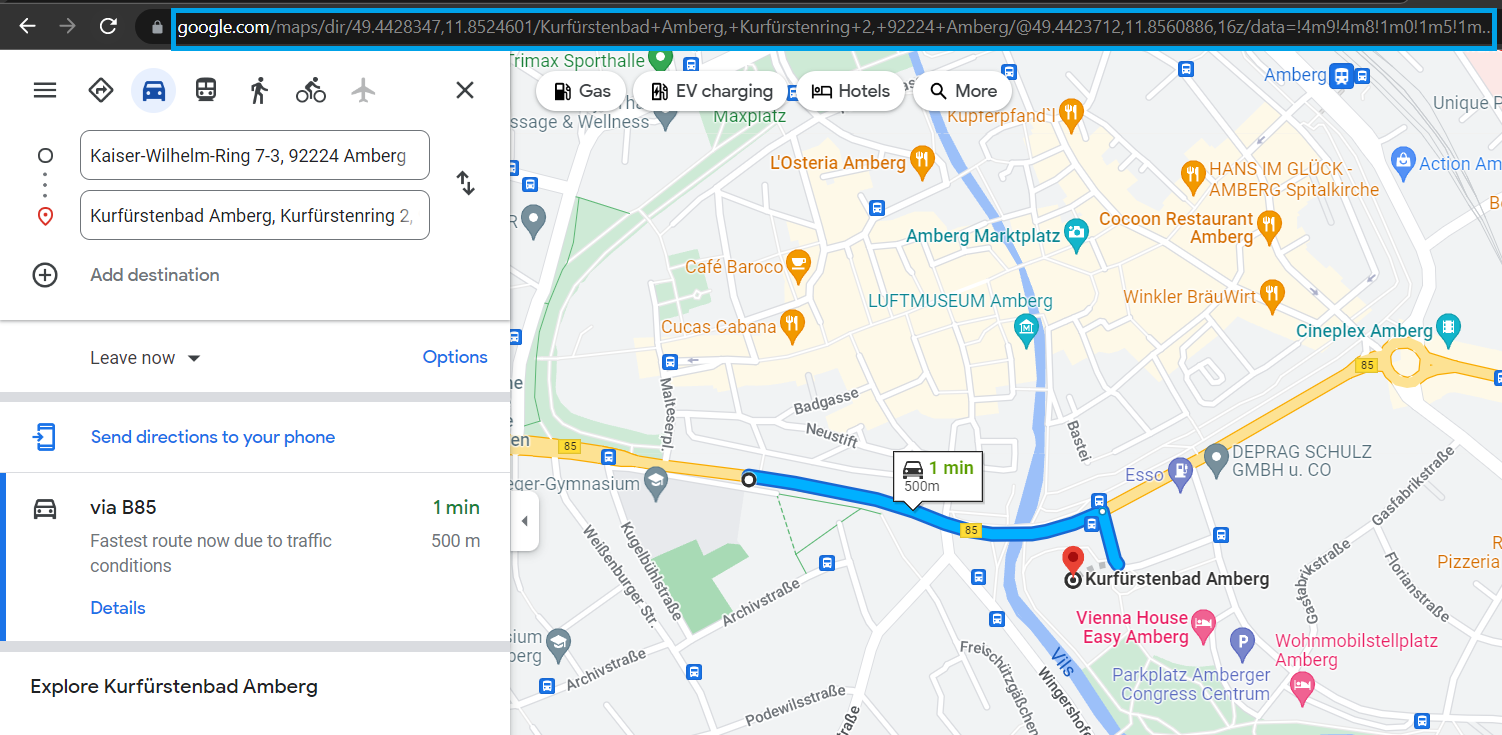
\includegraphics[scale=0.3]{img/path}
	\caption{Berechnung des Wegs zum nähesten Parkhaus von einem Punkt im Altstadtring mit markierter URL}
	\label{fig:path}
\end{wrapfigure}
Die Funktionen und Dateien der Navigation sind im Ordner \verb|Navigation| angesiedelt. Zentral für die Navigation ist die Datei \verb|findCorrectGpxFile.ts|. Diese Datei enthält Funktionen, welche eine Liste aus 48 GPX-Dateien analysiert und die richtige für die Navigation auswählt. Diese GPX-Dateien wurden per Hand erstellt, indem ein Punkt im Altstadtring auf der Karte ausgewählt wurde. Von diesem Punkt aus wurde durch die App das näheste Parkhaus über die Luftlinie, also wieder Haversine Distanz, berechnet. Mit diesen Daten wurde ein Pfad in Google Maps zum nähesten Parkhaus berechnet, wie in \autoref{fig:path} zu sehen ist. Die Informationen dieses Wegs werden in die URL geschrieben. Mithilfe eines Konvertierers können diese Informationen in eine GPX-Datei umgewandelt werden, die wiederum in die Karte der App durch das react-native-maps Paket über die Polyline-Komponente eingezeichnet werden können. Ein möglicher Konvertierer ist die ,,Maps to GPX Converter''-Webseite, welche den Google Maps Link annimmt und daraus eine GPX-Datei des Pfades erzeugt. Mit dieser Methode wurde einmal um den ganzen Altstadtring in 100 Meter Abständen der Weg zum nähesten Parkhaus berechnet. Das Ergebnis sind die oben erwähnten 48 GPX-Dateien, welche zudem noch in TypeScript-Dateien umgewandelt werden mussten, um diese für react-native verfügbar zu machen.

Um nun die richtige GPX-Datei zu finden, muss der Funktion \verb|findCorrectGpxFile| in der gleichnamigen Datei nur die Zielkoordinaten, also die Koordinaten des Parkhauses, zu dem navigiert werden soll, übergeben werden. Wenn diese Koordinaten 0 sind, wird automatisch zum nähesten Parkhaus navigiert. Die Suche nach der Datei zum nähesten Parkhaus läuft dann folgendermaßen ab: Zuerst erfragt die Funktion die aktuelle Position des Nutzer. Mit dieser Position wird die Entfernung zu allen Anfangspunkten der 48 GPX-Dateien über die Haversine Distanz berechnet. Wenn der Nutzer mehr als 100 Meter von allen Startpunkten der Dateien entfernt ist, ist die Navigation zu ungenau und der Nutzer wird zu Google Maps weitergeleitet. Falls es Startpunkte gibt, die weniger als 100 Meter entfernt sind, wird die GPX-Datei mit dem nähesten Startpunkt genommen. Diese GPX-Datei wird dann an die \verb|Directions.tsx|-Komponente im Ordner \verb|Map| übergeben, damit diese den Pfad in die Karte einzeichnet, was in \autoref{fig:navigation} gezeigt wird. Die Navigation lässt sich über den Knopf mit der Aufschrift ,,Abbrechen'' rechts unten beenden. Dabei wird nur die eingezeichnete Linie wieder aus der Karte gelöscht.

\begin{wrapfigure}{R}{0.5\textwidth}
	\vspace{-\baselineskip}
	\centering
	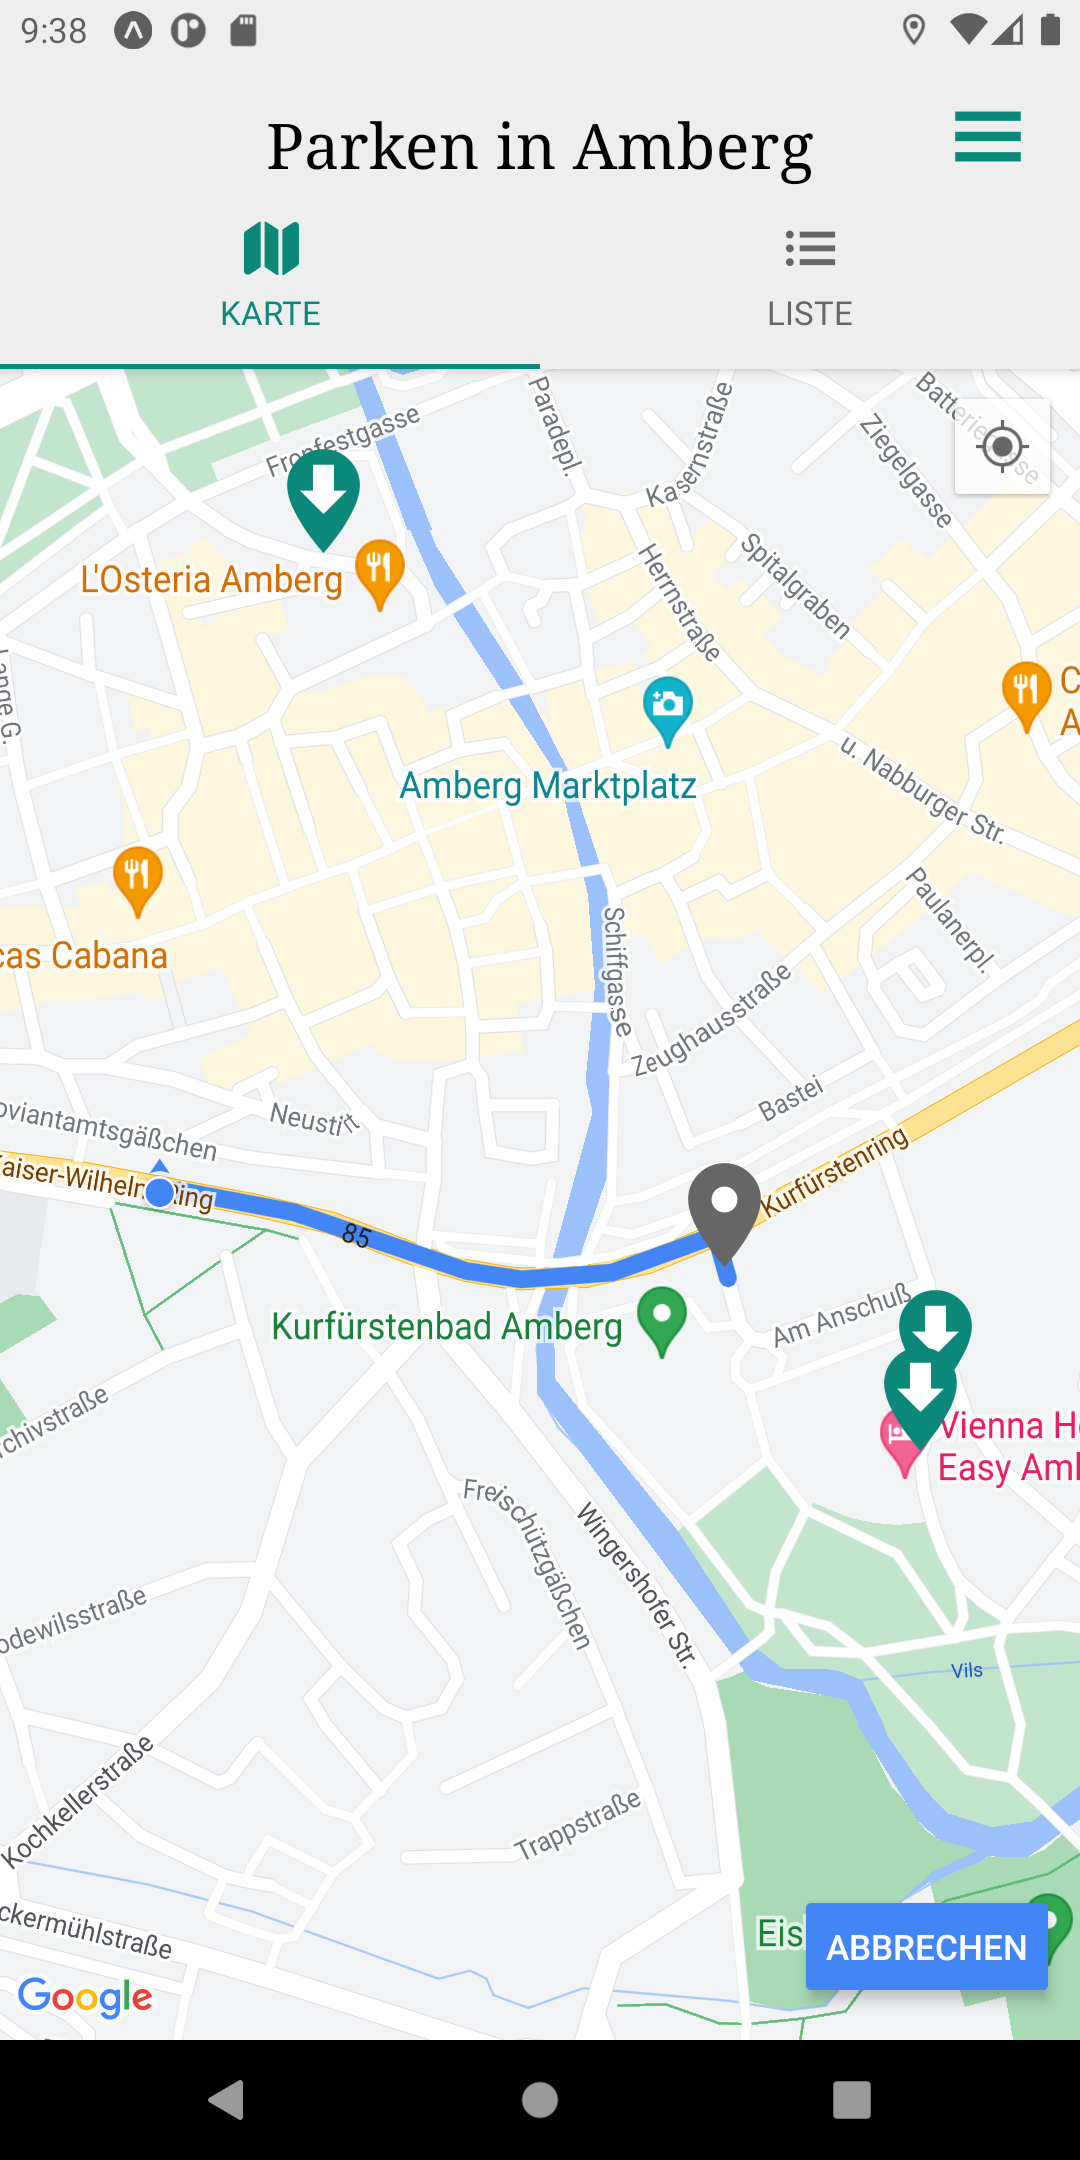
\includegraphics[scale=0.15]{img/navigation}
	\caption{Interne Navigation zum Kurfürstenbad über Einzeichnen der Daten einer GPX-Datei}
	\label{fig:navigation}
\end{wrapfigure}
Falls nun ein bestimmtes Parkhaus gefunden werden soll, wird wieder zuerst die Position des Nutzers erfragt. Danach werden die Entfernungen der Startpunkte der GPX-Dateien berechnet. Hier werden alle GPX-Dateien in einem Array gespeichert, deren Startpunkt weniger als 50 Meter vom Nutzer entfernt sind, da diese Navigation genauer sein soll. Dieses Array wird nun für die Endpunkte durchgegangen. Zu jedem Kandidaten der Dateien wird die Entfernung des Endpunkts zur gewünschten Zielkoordinate des Parkhauses berechnet. Falls ein Endpunkt einer Datei wieder weniger als 50 Meter von den Zielkoordinaten entfernt liegt, kann mit dieser GPX-Datei navigiert werden. Für mehr Genauigkeit wird hier wieder die Datei zum Einzeichnen in die Karte verwendet, deren Endpunkt den geringsten Abstand zum gewünschten Parkhaus besitzt. Falls keine Datei gefunden werden kann, wird wieder zu Google Maps weitergeleitet. Wenn jedoch die Einstellung ,,Immer Google Maps nutzen'' der Karte aktiviert ist, wird immer zu Google Maps weitergeleitet und diese Berechnungen finden nicht statt. Falls hier wieder keine Zielkoordinaten gegeben sind, wird in Google Maps zum nähesten Parkhaus navigiert, welches wieder über die Luftlinie berechnet wird. Im Falle, dass Koordinaten gegeben sind, wird zu diesen navigiert.

Die Weiterleitung zu Google Maps erfolgt über folgenden Link: \url{https://www.google.com/maps/dir/?api=1&destination="Latitude","Longitude"} \cite{MapsLinks}. Anstatt ,,Latitude'' und ,,Longitude'' müssen in diesen Link nur noch die Koordinaten des Ziels, also des Parkhauses, eingesetzt werden. Über diesen Link wird entweder zur Google Maps App weitergeleitet, falls diese auf dem Smartphone installiert und verfügbar ist, oder es wird Google Maps im Browser geöffnet. Durch den Zusatz \verb|/dir/| im Link wird bei Aufruf von Google Maps zudem auch die Navigation von der aktuellen Position des Nutzers zu den Zielkoordinaten im Link gestartet. Der Link wird von der App automatisch, wenn erforderlich, ausgeführt, um die Weiterleitung zu starten. Die Weiterleitung zu Google Maps wird dem Nutzer auch über eine Meldung gezeigt. Mit dieser Methode ist sichergestellt, dass der Nutzer von jeder Position aus zu einem Parkhaus navigieren kann, auch wenn er nicht auf dem Altstadtring ist. Falls der Nutzer jedoch auf dem Altstadtring ist, ist die Navigation angenehmer, da dann kein App-Wechsel stattfindet, sondern nur die Karte der App aufgerufen und der Pfad eingezeichnet wird.

Ein Nachteil der internen Navigation der App ist jedoch, dass die Startpunkte der GPX-Dateien manchmal einen sehr großen Abstand zum Nutzer aufweisen, besonders wenn nur zum nähesten Parkhaus navigiert werden soll, da hier der Abstand bis zu 100 Meter betragen darf. Hier müssten viel mehr GPX-Dateien angelegt werden, um eine größere Abdeckung des Altstadtrings zu erreichen. Als proof-of-concept ist diese Menge an GPX-Dateien jedoch ausreichend.

Die beschriebenen Berechnungen werden bei jedem Klick auf den Navigationspfeil entweder in der Karte oder im Detail-Fenster der Parkhäuser ausgeführt und eine Navigation findet somit entweder intern oder über Google Maps statt. Die Navigation zum nähesten Parkhaus erscheint hier überflüssig, wird jedoch für eine zusätzliche Funktion der App benötigt, welche im nächsten Kapitel beschrieben wird.
